\documentclass{ctexart}
\usepackage{PhysicalChemistryNote}

\begin{document}\pagestyle{plain}
\noindent\tbf{\LARGE 0A 极限,导数与微分}\vspace{15pt}\\
\indent 发展微积分的最初灵感之一来自试图去理解运动物体的速度,距离和时间的关系.%
人们经过数百年的探索建立了微积分这一学科,而这也是我们学习物理化学所必须掌握的数学基础知识.\vspace{12pt}\\
\Section{0A.1 极限\footnote{本节主要介绍的是函数极限.}}
\Part{极限的定义}
\indent 出于简单考虑,我们并不要求你了解极限的严格定义(即著名的$\ep-\delta$语言),而是通过一些更形象的方式理解极限的意义.%
尤其是考虑到我们遇见的函数大多具有良好的性质,因此直观的理解并不会出太多差错.\\
\indent 你也许遇到过这样的一些函数,它们在某些地方没有定义,但其值却会随着自变量向此处靠近而越来越接近某一值.例如下面的这个函数,$f(x)=x+1(x\in\R\backslash\left\{0\right\})$.
\begin{tightcenter}
    \documentclass{standalone}
\usepackage{PhysicalChemistryNote}
\begin{document}
\begin{tikzpicture}
	\draw[->] (-2,0)--(2,0) node[right]{$x$};
	\draw[->] (0,-2)--(0,2) node[above]{$f(x)$};
	\draw[-,thick,blue] (-1.5,-1)--(1.5,2);
	\draw[fill=white] (0,0.5) circle (1.5pt);
\end{tikzpicture}
\end{document}
\end{document}
\end{tightcenter}

\indent 尽管$f(x)$在$x=0$处没有定义,但你可以从图像上发现当$x$逐渐接近$0$时,$f(x)$也逐渐接近$1$.%
因此,尽管$f(x)$在$x=0$处没有定义,我们也可以获知$x$逐渐接近于$0$时$f(x)$的变化情况.因此,我们可以尝试用自然语言描述极限的定义.
\begin{definition}[0A.1.1 函数极限]
    当自变量$x$\tbf{无限接近}某一点$a$时,如果函数$f(x)$能\tbf{无限接近}于某一定值$l$,则称$f(x)$在$x=a$处的极限为$l$,记作
    \[\lim_{x\to a}f(x)=l\]
    这个定义的核心是描述函数在某个点附近的\tbf{趋势},而不是该点的具体值.
\end{definition}
定义中的无限接近是由$\ep-\delta$语言保证的,但你并不需要了解这一点,只需对极限有一个直观认识即可.
\begin{hint}
    值得注意的是,$f(x)$在$x=0$附近对$1$的接近是任意的:对于任意$\ep>0$,总存在$x=0$附近的一个区间$(-\delta,\delta)\backslash\{0\}$%
    使得这一区间内的所有$x$都满足$\left|f(x)-1\right|<\ep$.这就是极限的$\ep-\delta$语言.
\end{hint}
\Part{连续函数}
\indent 你也许听说过\tbf{连续}这一概念.想象用笔在纸上画一条曲线.%
如果你在绘制的过程中笔尖始终接触纸面,线条不间断,那么从直觉来说你应该画出了一条连续的曲线.%
反之,如果你在绘制的过程中笔尖离开了纸面,从而出现了跳跃或间断点,那么这条曲线就应当是不连续的.%
我们可以观察下面的几个函数.
\begin{tightcenter}
    \documentclass{standalone}
\usepackage{PhysicalChemistryNote}
\begin{document}
\begin{tikzpicture}
	\draw[->] (-2,0)--(2,0) node[right]{$x$};
	\draw[->] (0,-2)--(0,2) node[above]{$f_1(x)$};
	\draw[-,thick,blue] (-1.5,-1)--(1.5,2);
	\draw[fill=white] (0,0.5) circle (1.5pt);
\end{tikzpicture}
\begin{tikzpicture}
	\draw[->] (-2,0)--(2,0) node[right]{$x$};
	\draw[->] (0,-2)--(0,2) node[above]{$f_2(x)$};
	\draw[-,thick,blue] (-1.5,-2)--(0,-0.5);
	\draw[-,thick,blue] (0,0.5)--(1.5,2);
	\draw[fill=white] (0,0.5) circle (1.5pt);
	\draw[fill=white] (0,-0.5) circle (1.5pt);
	\fill (0,0) circle (1.5pt);
\end{tikzpicture}
\begin{tikzpicture}
	\draw[->] (-2,0)--(2,0) node[right]{$x$};
	\draw[->] (0,-2)--(0,2) node[above]{$f_3(x)$};
	\draw[-,thick,blue] (-1.5,-1)--(1.5,2);
\end{tikzpicture}
\end{document}
\end{document}
\end{tightcenter}

\indent $f_1(x)$在$x=0$处没有定义,即出现了一个间断点,应当是不连续的.%
$f_2(x)$虽然在$x=0$处有定义,但其在$x=0$处的左侧极限和右侧极限不相等,也与$f_2(0)$不相等,函数出现了跳跃,也是不连续的.%
只有$f_3(x)$满足在$x=0$处有定义,且左侧极限和右侧极限均与定义的函数值相等,这在图像上表现为一段连续不断的曲线.%
这就是连续函数的定义.
\begin{definition}[0A.1.2 连续与连续函数]
    如果函数$f(x)$在$x=a$处有定义,并且在$x=a$处的两侧的极限均等于$f(a)$,即
    \[\lim_{x\to a}f(x)=f(a)\]
    那么就称$f(x)$在$x=a$处\tbf{连续}.\\
    如果$f(x)$在其定义域上的每一点都连续,那么就称$f(x)$为其定义域上的\tbf{连续函数}.
\end{definition}
常见的函数,例如多项式函数,三角函数,指对数函数等初等函数均在其定义域上连续.这一性质同样对初等函数的复合函数也成立.\vspace{4pt}\\
\Part{夹逼准则与极限的运算\footnote{本节仅作介绍,不必要求掌握.了解本节的内容有助于理解导数的计算过程.}}
\indent 我们先来介绍夹逼准则.
\begin{theorem}[0A.1.3 夹逼准则]
    对于函数$f_1(x),f_2(x),f_3(x)$和给定的$a$,如果在包含$a$的区间上总有$f_1(x)\leqslant f_2(x)\leqslant f_3(x)$,并且
    \[\lim_{x\to a}f_1(x)=\lim_{x\to a}f_3(x)=l\]
    那么一定有
    \[\lim_{x\to a}f_2(x)=l\]
    
\end{theorem}
直观地说,因为$f_1(x)$和$f_3(x)$都趋近于$l$,因此被夹在它们中间的$f_2(x)$也只能被迫趋近于$l$.%
我们以一个简单的例子对其进行直观理解.
\begin{problem}[P.0A.1]
    求极限$\displaystyle\lim_{x\to0}x\sin\dfrac1x$.
\end{problem}
\begin{solution}
    目标函数$f(x)=x\sin\dfrac1x$在$x=0$处没有定义,因此不能使用连续函数的性质解决问题.然而,我们可以注意到
    \[-1\leqslant \sin\dfrac1x\leqslant 1\]
    对所有$x\in\R\backslash\{0\}$成立,因此有
    \[-x<x\sin\dfrac1x<x\]
    而
    \[\lim_{x\to0}(-x)=\lim_{x\to0}x=0\]
    这是由连续函数的性质决定的.因此,我们可以得出
    \[\lim_{x\to0}x\sin\dfrac1x=0\]
    观察图像,可以发现$f(x)=x\sin\dfrac1x$被夹在$g(x)=x$和$h(x)=-x$之间,而后两个函数在$x$趋近于$0$时都趋近于$0$.%
    自然,$f(x)$也被迫趋向于$0$.夹逼准则可以解决许多难以计算的极限问题.
    \begin{tightcenter}
        \documentclass{standalone}
\usepackage{PhysicalChemistryNote}
\begin{document}
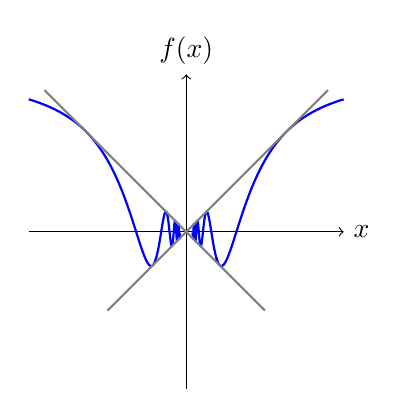
\begin{tikzpicture}[scale=2]
	\draw[->] (-1,0)--(1,0) node[right]{$x$};
	\draw[->] (0,-1)--(0,1) node[above]{$f(x)$};
	\draw[-,blue,thick,domain=-1:-0.19]plot[samples=400](\x,{\x*sin(180/(\x*pi))});
	\draw[-,blue,thick,domain=-0.2:-0.04]plot[samples=1000](\x,{\x*sin(180/(\x*pi))});
	\draw[-,blue,thick,domain=0.19:1]plot[samples=400](\x,{\x*sin(180/(\x*pi))});
	\draw[-,blue,thick,domain=0.04:0.2]plot[samples=1000](\x,{\x*sin(180/(\x*pi))});
	\draw[-,thick,gray,domain=-0.5:0.9] plot[smooth](\x,\x);
	\draw[-,thick,gray,domain=-0.9:0.5] plot[smooth](\x,-\x);
\end{tikzpicture}
\end{document}
\end{document}
    \end{tightcenter}
    
\end{solution}
除了使用夹逼准则以外,我们还可以利用极限的四则运算和复合来计算复杂函数的极限.
\begin{theorem}[0A.1.4 极限的四则运算]
    如果$f(x)$和$g(x)$满足
    \[\lim_{x\to a}f(x)=l_1\ \ \ \ \ \lim_{x\to a}g(x)=l_2\]
    那么我们有
    \[\lim_{x\to a}f(x)\pm g(x)=\l_1\pm l_2\]
    \[\lim_{x\to a}f(x)\cdot g(x)=l_1l_2\]
    \[\lim_{x\to a}\dfrac{f(x)}{g(x)}=\dfrac{l_1}{l_2}\left(l_2\neq0\right)\]
    即如果两个函数在某处的极限均存在,那么这两个函数的四则运算所得的函数在此处的极限亦存在,并且其值等于各自的极限值进行相应的四则运算的结果.
\end{theorem}
\begin{theorem}[0A.1.5 复合函数的极限]
    如果$\displaystyle\lim_{x\to a}f(x)=l$,而$g(x)$在$x=l$及其附近的区间上连续,那么
    \[\lim_{x\to a}g(f(x))=g(l)\]
    这就是说,如果复合函数的外部连续(这一条件是容易满足的),就可以先对内部求极限后代入外部函数从而得到总体的极限值.%
    这意味着我们可以对极限进行换元以简化计算.
\end{theorem}
上面两个定理的证明较为繁琐,因此你不必掌握它们的证明方法.总之,极限运算(在我们目前能接触到的函数中)%
是十分符合常理的.\vspace{4pt}\\
\Part{两个重要极限}
\indent 在日后的学习中,你经常会遇到自然常数$\e$.它是由下面的式子定义的.
\begin{definition}[0A.1.6 自然常数]
    自然常数$\e$定义为
    \[\e=\lim_{x\to+\infty}\left(1+\dfrac1x\right)^x\]
    与我们在前面定义的极限不同的是,这里的$x\to+\infty$表示$x$趋向于正无穷大,而整个式子将趋向于定值$\e$.
\end{definition}
关于其独特而重要的性质,主要体现在日后微积分的应用中,我们将在到时进行详细叙述.\\
\indent 另一个重要的极限是关于三角函数的.这一极限的存在将在三角函数的微积分中发挥重要作用.
\begin{theorem}[0A.1.7 重要极限II]
    我们有
    \[\lim_{x\to0}\dfrac{\sin x}{x}=1\]

\end{theorem}
\begin{proof}
    相信你应当在初中学习三角函数时知道
    \[\sin x<x<\tan x,\forall x\in\left(0,\dfrac\pi2\right)\]
    稍作变形即可得到
    \[\cos x<\dfrac{\sin x}{x}<1\]
    由于$\displaystyle\lim_{x\to0}\cos x=1$(因为$\cos x$是连续函数),因而根据夹逼定理可得
    \[\lim_{x\to0}\dfrac{\sin x}{x}=1\]

\end{proof}
\begin{hint}
    严格来说,上述证明有循环论证之嫌,这取决于我们定义三角函数的方式.避免这样的逻辑问题的方式是采取复分析的方法定义三角函数,%
    不过这显然超出了我们的知识水平.如果你对这一问题感兴趣,可以自行查阅相关资料.
\end{hint}
\Section{0A.2 导数}
\Part{导数的定义}
\indent 应该来说,前一节的内容都是非必须的,只是让你对导数所涉及的极限运算有一个大致的认识.%
或者更确切地说,这一章节的内容都是为了让你对微积分有一个简单的,偏向直观的了解,而非与那些性质古怪的函数打交道.
\begin{hint}
    初等函数(即本书所讨论的绝大多数函数)都是光滑的.这在图像上表现为一条“看起来”光滑的曲线,不仅连续,而且没有粗糙的折点.%
    一个函数光滑意味着它具有良好的性质,我们可以不加考虑地对它进行求导,无需担心可能出现的差错或意外.
\end{hint}
正如前言中所说,人们是从物体的运动状态开始研究微积分的.在初中时,你应当学过简单的运动学知识:在一段时间$t$内,物体运动的距离\footnote{准确而言应当是位移.此处我们假定物体做直线运动,因而位移就与距离的数值相同.}%
$x$与$t$之比就是它在这段时间内的平均速度$v$,即
\[v=\dfrac xt\]
我们让这段时间从某一时间点$t_0$开始,并结束于$t_0+\Delta t$,在这段时间内物体运动的距离为$\Delta x$.于是这段时间内的平均速度为
\[\bar{v}=\dfrac{\Delta x}{\Delta t}\]
为了考虑物体在某一时间点$t_0$时的运动状态,我们尝试用求极限的方式求出$t_0$时的速度的极限值.%
令$\Delta t$越来越小.在此过程中,物体的平均速度$\bar{v}$应当趋近于某一定值,这就是某一时间$t_0$时该物体的瞬时速度$v_0$,可以记为
\[v_0=\lim_{\Delta t\to 0}\dfrac{\Delta x}{\Delta t}\]
某一时间$t_0$的瞬时速度$v_0$等于当$\Delta t$趋近于$0$时$\left(t_0,t_0+\Delta t\right)$时间段内的运动距离$\Delta x$与$\Delta t$之比值的极限.%
我们知道,速度即为运动距离对时间的变化率.上面的叙述就可以引出导数的(浅显而形象的)定义.
\begin{definition}[0A.1.1 导数]
    函数$y=f(x)$在$x=x_0$处的导数定义为
    \[f'\left(x_0\right)=\lim_{\Delta x\to 0}\dfrac{f\left(x+\Delta x\right)-f(x)}{\Delta x}\]
    在各点处的$f'\left(x_0\right)$亦可以构成一个新的函数,这一函数$f'(x)$记为$f(x)$的导函数.%
    今后,我们说某一函数的导数,一般就指其导函数.
\end{definition}
上述的介绍难免有些粗略而晦涩.%
如果你想对高等数学的内容有更加深入的了解,笔者建议你阅读普林斯顿微积分读本以获得对微积分的初步认识,然后再阅读各种高等数学书籍.\vspace{4pt}\\
\Part{常见函数的导数}
\indent 接下来,我们将从定义出发推导一些函数的导函数.首先是简单的幂函数.
\begin{problem}[P.0A.2]
    求函数$f(x)=x$的导函数.
\end{problem}
\begin{derivation}
    我们有
    \[f'(x)=\lim_{\Delta x\to0}\dfrac{f(x+\Delta x)-f(x)}{\Delta x}
    =\lim_{\Delta x\to0}\dfrac{x+\Delta x-x}{\Delta x}=\lim_{\Delta x\to0}1=1\]
    因此$f(x)=x$的导函数为$f'(x)=1$.\\
    需要注意的是,上述极限中的变量为$\Delta x$,而$x$是一个固定的值.%
    我们所做的事实上是对每个给定的$x$(视作常数)求出此时的导数值,然后将所有$x$对应的导数值合并成一个导函数.%
    上面的式子把这两个过程合并在了一起,而你应当清楚地了解$x$和$\Delta x$各自的含义.
\end{derivation}
\begin{problem}[P.0A.3]
    求函数$f(x)=x^2$的导函数.
\end{problem}
\begin{derivation}
    同样地,我们有
    \[\begin{aligned}
        f'(x)
        &= \lim_{\Delta x\to0}\dfrac{f(x+\Delta x)-f(x)}{\Delta x}=\lim_{\Delta x\to0}\dfrac{(x+\Delta x)^2-x^2}{\Delta x} \\
        &= \lim_{\Delta x\to0}\dfrac{2x\Delta x-(\Delta x)^2}{\Delta x}=\lim_{\Delta x\to0}(2x+\Delta x)=2x
    \end{aligned}\]
    因此$f(x)=x^2$的导函数为$f'(x)=2x$.\\
    在微积分被发明出来的一段时间内,导数并没有经由极限这一概念进行严格定义.%
    Bishop Berkeley把$\Delta x$称作“消逝的量的鬼魂”,因为它既可以作为除数,又在最后作为无穷小量被舍弃.%
    这一困境在Cauchy提出极限的概念之后才得以解决.现在我们知道,我们从来都没有把$\Delta x$看作是$0$,%
    只是考察整个式子在$\Delta x\to0$时所趋近的值.只不过大部分时候由连续函数的性质,%
    我们可以在最后把$\Delta x=0$代入以方便地得到最终的结果.%
    这和直接令$\Delta x=0$是有本质区别的.
\end{derivation}
\begin{problem}[P.0A.4]
    求函数$f(x)=\dfrac1x$的导函数.
\end{problem}
\begin{derivation}
    我们有
    \[\begin{aligned}
        f'(x)
        &= \lim_{\Delta x\to0}\dfrac{f(x+\Delta x)-f(x)}{\Delta x}=\lim_{\Delta x\to0}\dfrac{\frac{1}{x+\Delta x}-\frac1x}{\Delta x} \\
        &= \lim_{\Delta x\to0}\dfrac{1}{\Delta x}\cdot\dfrac{x-(x+\Delta x)}{x(x+\Delta x)}=-\lim_{\Delta x\to0}\dfrac{1}{x^2+x\Delta x} \\
        &= -\dfrac1{x^2}
    \end{aligned}\]
    于是$f(x)=\dfrac1x$的导函数为$f'(x)=-\dfrac{1}{x^2}$.
\end{derivation}
\begin{problem}[P.0A.5]
    求函数$f(x)=\sqrt{x}$的导函数.
\end{problem}
\begin{derivation}
    我们有
    \[\begin{aligned}
        f'(x)
        &= \lim_{\Delta x\to0}\dfrac{f(x+\Delta x)-f(x)}{\Delta x}=\lim_{\Delta x\to0}\dfrac{\sqrt{x+\Delta x}-\sqrt{x}}{\Delta x} \\
        &= \lim_{\Delta x\to0}\dfrac{(x+\Delta x)-x}{\left(\sqrt{x+\Delta x}+\sqrt{x}\right)\Delta x} \\
        &= \lim_{\Delta x\to0}\dfrac{1}{\sqrt{x+\Delta x}+\sqrt{x}} \\
        &= \dfrac{1}{2\sqrt{x}}
    \end{aligned}\]
    于是$f(x)=\sqrt{x}$的导函数为$f'(x)=\dfrac{1}{2\sqrt{x}}$.
\end{derivation}
经过总结与归纳(严格的证明需要用到广义二项展开,这里就不再介绍),%
我们可以得出幂函数$f(x)=x^a$的导函数的通式.
\begin{theorem}[0A.2.2 幂函数的导数]
    幂函数$f(x)=x^a(a\in\R)$的导函数为$f'(x)=ax^{a-1}$.
\end{theorem}
接下来是常见的三角函数.
\begin{problem}[P.0A.6]
    求函数$f(x)=\sin x$的导函数.
\end{problem}
\begin{derivation}
    根据简单的和差角公式,我们可以得到
    \[\begin{aligned}
        f'(x)
        &= \lim_{\Delta x\to0}\dfrac{f(x+\Delta x)-f(x)}{\Delta x}=\lim_{\Delta x\to0}\dfrac{\sin(x+\Delta x)-\sin{x}}{\Delta x} \\
        &= \lim_{\Delta x\to0}\dfrac{\sin x\cos\Delta x+\sin\Delta x\cos x-\sin x}{\Delta x} \\
        &= \lim_{\Delta x\to0}\dfrac{\sin x(1-\cos\Delta x)}{\Delta x}+\lim_{\Delta x\to0}\dfrac{\cos x\sin\Delta x}{\Delta x} \\
    \end{aligned}\]
    现在我们分别处理这两个极限.我们有
    \[\begin{aligned}
        \lim_{\Delta x\to0}\dfrac{1-\cos\Delta x}{\Delta x}
        &= \lim_{\Delta x\to0}\dfrac{\left(1-\cos\Delta x\right)\left(1+\cos\Delta x\right)}{\Delta x\left(1+\cos\Delta x\right)} \\
        &= \lim_{\Delta x\to0}\dfrac{1-\cos^2\Delta x}{\Delta x\left(1+\cos\Delta x\right)} \\
        &= \lim_{\Delta x\to0}\dfrac{\sin\Delta x}{\Delta x}\cdot\lim_{\Delta x\to0}\dfrac{\sin\Delta x}{1+\cos\Delta x} \\
        &= 1\cdot0=0
    \end{aligned}\]
    而后一项即为我们在前面所述的重要极限.因此有
    \[f'(x)=\sin x\cdot 0+\cos x\cdot 1=\cos x\]
    于是$f(x)=\sin x$的导函数为$f'(x)=\cos x$.
\end{derivation}
\begin{problem}[P.0A.7]
    求函数$f(x)=\cos x$的导函数.
\end{problem}
\begin{derivation}
    方法是与正弦函数完全一致的.我们有
    \[\begin{aligned}
        f'(x)
        &= \lim_{\Delta x\to0}\dfrac{f(x+\Delta x)-f(x)}{\Delta x}=\lim_{\Delta x\to0}\dfrac{\cos(x+\Delta x)-\cos{x}}{\Delta x} \\
        &= \lim_{\Delta x\to0}\dfrac{\cos x\cos\Delta x-\sin\Delta x\sin x-\cos x}{\Delta x} \\
        &= \lim_{\Delta x\to0}\dfrac{\cos x(1-\cos\Delta x)}{\Delta x}-\lim_{\Delta x\to0}\dfrac{\sin x\sin\Delta x}{\Delta x} \\
        &= -\sin x
    \end{aligned}\]
    于是$f(x)=\cos x$的导函数为$f'(x)=-\sin x$.
\end{derivation}
最后是指数函数与对数函数.这两类函数相比前面的两类函数则略为复杂.
\begin{problem}[P.0A.8]
    求函数$f(x)=a^x(a>0)$的导函数.
\end{problem}
\begin{derivation}
    按照定义,我们有
    \[f'(x)=\lim_{\Delta x\to0}\dfrac{a^{x+\Delta x}-a^x}{\Delta x}=a^x\lim_{\Delta x\to0}\dfrac{a^{\Delta x}-1}{\Delta x}\]
    后面的极限值看起来是一个较难处理的函数.我们可以做换元$t=a^{\Delta x}-1$,这样就有$\Delta x=\log_a(t+1)$.于是我们有
    \[\lim_{\Delta x\to0}\dfrac{a^{\Delta x}-1}{\Delta x}=\lim_{t\to0}\dfrac{t}{\log_a(t+1)}
    =\lim_{t\to0}\dfrac{1}{\log_a\left(1+t\right)^{\frac1t}}\]
    注意到这和我们定义的自然常数的相似性.因此,可以再令$s=\dfrac1t$,于是
    \[\lim_{t\to0}\left(1+t\right)^{\frac1t}=\lim_{s\to0}\left(1+\dfrac1s\right)^s=\e\]
    因此
    \[\lim_{\Delta x\to0}\dfrac{a^{\Delta x}-1}{\Delta x}=\dfrac{1}{\log_a\e}=\ln a\]
    于是$f(x)=a^x$的导函数为$f'(x)=a^x\ln x$.特别地,当$a=\e$时,就有$f(x)=f'(x)=\e^x$.%
    这也是自然常数体现出的特殊性质之一.
\end{derivation}
\begin{problem}[P.0A.9]
    求函数$f(x)=\log_ax(a>0)$的导函数.
\end{problem}
\begin{derivation}
    我们有
    \[\begin{aligned}
        f'(x)
        &= \lim_{\Delta x\to0}\dfrac{\log_a(x+\Delta x)-\log_a x}{\Delta x} \\
        &= \lim_{\Delta x\to0}\dfrac1x\cdot\dfrac{x}{\Delta x}\cdot\log_a\left(1+\dfrac{\Delta x}{x}\right) \\
        &= \lim_{\Delta x\to0}\dfrac1x\log_a\left(1+\dfrac{\Delta x}{x}\right)^{\frac{x}{\Delta x}} \\
        &\xlongequal{u=\frac{\Delta x}{x}} \dfrac1x\lim_{u\to0}\log_a(1+u)^{\frac1u} \\
        &= \dfrac{\log_a\e}{x} = \dfrac{1}{x\ln a}
    \end{aligned}\]
    于是$f(x)=\log_a x$的导函数为$f'(x)=\dfrac{1}{x\ln a}$.特别地,当$a=\e$时$f(x)=\ln x$,%
    $f'(x)=\dfrac1x$.
\end{derivation}
\Part{导(函)数的运算法则}
\indent 导函数的运算法则是十分重要且基础的工具.它能让我们从简单的函数出发直接推出复杂函数的导函数,%
而无需通过定义求导.这避免了繁琐的极限运算.事实上,即使不清楚初等函数的导函数的由来,%
我们仍然可以通过记忆它们的导函数,再通过导函数的运算法则求出许多函数的导函数.
\begin{theorem}[0A.1.2]
    导函数的运算法则主要有以下几条.
    \begin{enumerate}[label=\tbf{\roman*.},topsep=0pt,parsep=0pt,itemsep=0pt,partopsep=0pt]
        \item \tbf{导数的加减法}\\如果$h(x)=f(x)\pm g(x)$,那么$h'(x)=f'(x)\pm g'(x)$.
        \item \tbf{导数的乘法}\\如果$h(x)=f(x)g(x)$,那么$h'(x)=f'(x)g(x)+f(x)g'(x)$.
        \item \tbf{导数的除法}\\如果$h(x)=\dfrac{f(x)}{g(x)}$,那么$h'(x)=\dfrac{f'(x)g(x)-f(x)g'(x)}{(g(x))^2}$
        \item \tbf{导数的复合}\\如果$h(x)=f(g(x))$,那么$h'(x)=f'(g(x))\cdot g'(x)$.
    \end{enumerate}
\end{theorem}
以下是这些运算法则的简单说明.
\begin{proof}
    导函数的加减法是容易理解的.\\
    为了说明导数的乘法,我们考虑如下变换.
    \[\begin{aligned}
        &h(x+\Delta x)-h(x)\\
        =&f(x+\Delta x)g(x+\Delta x)-f(x)g(x) \\
        =&\left(f(x+\Delta x)-f(x)+f(x)\right)\left(g(x+\Delta x)-g(x)+g(x)\right)-f(x)g(x) \\
        =&\left(f(x+\Delta x)-f(x)\right)\left(g(x+\Delta x)-g(x)\right)\\
        &+f(x)\left(g(x+\Delta x)-g(x)\right)+g(x)\left(f(x+\Delta x)-f(x)\right)
    \end{aligned}\]
    因此我们有
    \[\begin{aligned}
        h'(x)
        &= \lim_{\Delta x\to0}\dfrac{h(x+\Delta x)-h(x)}{\Delta x} \\
        &= f(x)g'(x)+f'(x)g(x)+\lim_{\Delta x\to0}\Delta x\cdot\dfrac{f(x+\Delta x)-f(x)}{\Delta x}\cdot\dfrac{g(x+\Delta x)-g(x)}{\Delta x} \\
        &= f(x)g'(x)+f'(x)g(x)+f'(x)g'(x)\cdot\lim_{\Delta x\to0}\Delta x \\
        &= f(x)g'(x)+f'(x)g(x)
    \end{aligned}\]
    这一推导还有一个形象一些的理解.
    \begin{tightcenter}
        \documentclass{standalone}
\usepackage{PhysicalChemistryNote}
\begin{document}
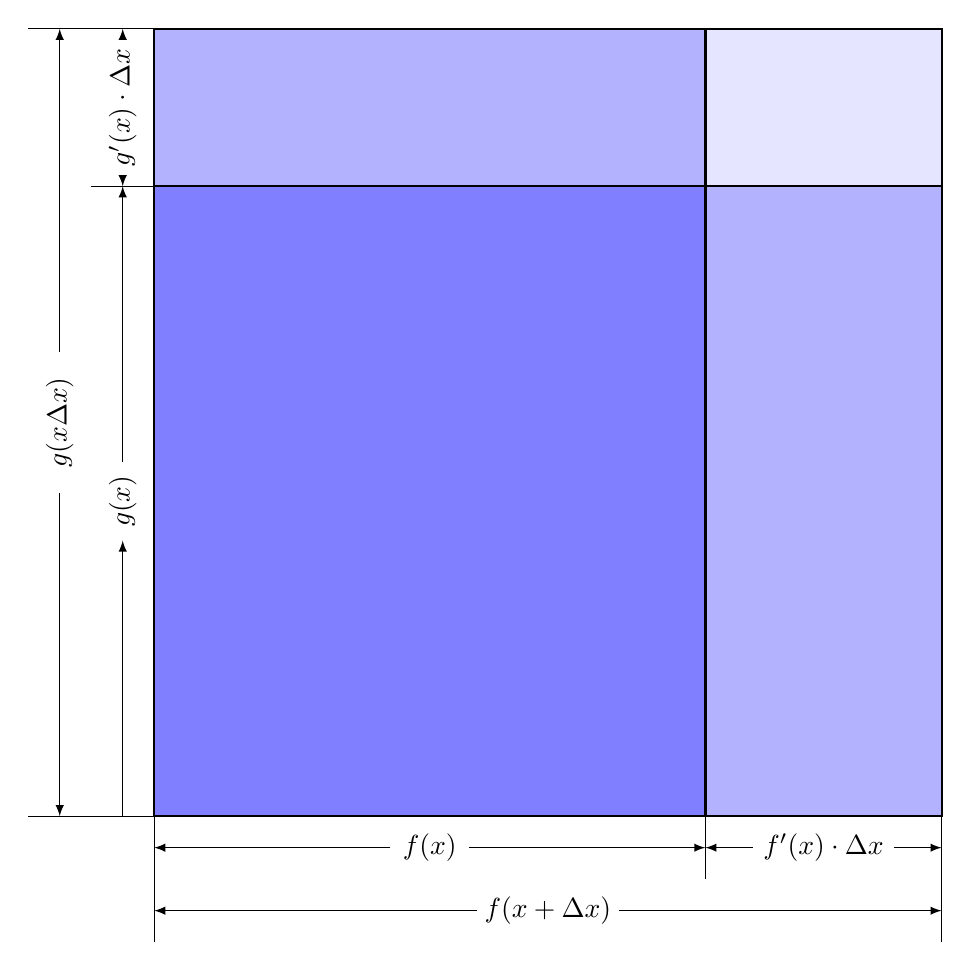
\begin{tikzpicture}[scale=2]
	\fill[blue,opacity=0.5] (0,0)rectangle(3.5,4);
	\fill[blue,opacity=0.3] (0,4)rectangle(3.5,5);
	\fill[blue,opacity=0.3] (3.5,0)rectangle(5,4);
	\fill[blue,opacity=0.1] (3.5,4)rectangle(5,5);
	\draw[-,thick] (0,0)--(5,0)--(5,5)--(0,5)--(0,0);
	\draw[-] (0,0)--(-0.4,0);
	\draw[-] (0,4)--(-0.4,4);
	\draw[-] (0,5)--(-0.5,5);
	\draw[-,thick] (0,4)--(5,4);
	\draw[-,thick] (3.5,0)--(3.5,5);
	\draw[-] (0,0)--(0,-0.8);
	\draw[-] (3.5,0)--(3.5,-0.4);
	\draw[-] (5,0)--(5,-0.8);
	\node at (1.75,-0.2) {$f(x)$};
	\node at (4.25,-0.2) {$f'(x)\cdot\Delta x$};
	\node at (2.5,-0.6) {$f(x+\Delta x)$};
	\draw[-latex] (1.5,-0.2)--(0,-0.2);
	\draw[-latex] (2,-0.2)--(3.5,-0.2);
	\draw[-latex] (3.8,-0.2)--(3.5,-0.2);
	\draw[-latex] (4.7,-0.2)--(5,-0.2);
	\draw[-latex] (2.05,-0.6)--(0,-0.6);
	\draw[-latex] (2.95,-0.6)--(5,-0.6);
	\draw[-] (0,0)--(-0.8,0);
	\draw[-] (0,5)--(-0.8,5);
	\draw[-] (0,4)--(-0.4,4);
	\node[rotate=90] at (-0.2,2) {$g(x)$};
	\node[rotate=90] at (-0.2,4.5) {$g'(x)\cdot\Delta x$};
	\node[rotate=90] at (-0.6,2.5) {$g(x\Delta x)$};
	\draw[-latex] (-0.6,2.05)--(-0.6,0);
	\draw[-latex] (-0.6,2.95)--(-0.6,5);
	\draw[-latex] (-0.2,0)--(-0.2,1.75);
	\draw[-latex] (-0.2,2.25)--(-0.2,4);
	\draw[-latex] (-0.2,4.95)--(-0.2,5);
	\draw[-latex] (-0.2,4.05)--(-0.2,4);
\end{tikzpicture}
\end{document}
\end{document}
    \end{tightcenter}
    可以看到,$h(x+\Delta x)$相比$h(x)$增加的部分即为图中的三个淡色的长方形的部分.%
    它们的面积分别为$f(x)g'(x)\Delta x$,$f'(x)g(x)\Delta x$和$f'(x)g'(x)(\Delta x)^2$.%
    当$\Delta x\to0$时,由于最后一项含有两个$\Delta x$,因此是相比前两项是可以忽略的无穷小量.%
    这样与$\Delta x$做比之后求极限即可得到结果.\\
    而复合函数的链式求导法则可以简单地解释如下.例如函数$y=h(x)$由函数$y=f(u),u=g(x)$复合而成.%
    粗略而言,导数总是变化率,因此给定增量$\Delta x$后,首先被函数$u=g(x)$作用,增量放大了$g'(x)$倍,即
    \[\dfrac{\Delta u}{\Delta x}\approx g'(x)\]
    然后$\Delta u$又在$f(u)$的作用下被放大了$f'(u)$倍,即
    \[\dfrac{\Delta y}{\Delta u}\approx f'(u)\]
    于是整体地看,$\Delta x$在复合函数$y=f(g(x))$的作用下被放大了
    \[f'(u)g'(x)\]
    倍,即
    \[\dfrac{\Delta y}{\Delta x}\approx f'(u)g'(x)=f'(g(x))\cdot g'(x)\]
    这就是链式法则的直观解释.上述等号是可以通过极限的知识进行严格证明的,这里就不再详细讨论了.\\
    导数的除法规则可以由链式法则和乘法规则共同推出.具体而言,你可以根据链式法则先求出$\dfrac{1}{g(x)}$%
    的导数为$-\dfrac{g'(x)}{\left(g(x)\right)^2}$,然后根据乘法规则即可得出最终的结果.
\end{proof}
我们来看一些简单的例题以巩固前面所学的知识.
\begin{exercise}[E.0A.1]
    求函数$f(x)=\e^x(\sin x+\cos x)$的导函数.
\end{exercise}
\begin{solution}
    $f(x)$可以看作是由$g(x)=\e^x$和$h(x)=\sin x+\cos x$相乘得到.因此
    \[f'(x)=\e^x(\sin x+\cos x)+\e^x(\cos x-\sin x)=2\e^x\cos x\]

\end{solution}
\begin{exercise}[E.0A.2]
    求函数$f(x)=\ln\left(x^2+1\right)$的导函数.
\end{exercise}
\begin{solution}
    $f(x)$可以看作是$g(u)=\ln u$和$u=h(x)=x^2+1$复合而成.因此
    \[f'(x)=\dfrac{1}{u}\cdot 2x=\dfrac{2x}{x^2+1}\]
    
\end{solution}
\begin{exercise}[E.0A.3]
    求函数$f(x)=x^x$的导函数.
\end{exercise}
\begin{solution}
    注意到$f(x)=x^x=\e^{x\ln x}$.因此可以将其视作复合函数,就有
    \[f'(x)=\e^{x\ln x}\cdot(\ln x+1)=x^x\left(\ln x+1\right)\]

\end{solution}
接下来,我们将讨论在微积分中的一个重要的概念:微分.\vspace{12pt}\\
\Section{0A.3 微分}
\Part{无穷小量与微分}
\indent 顾名思义,无穷小量就是以$0$为极限的变量.
\begin{definition}[0A.3.1 无穷小量]
    假定变量$y$与变量$x$具有函数关系$y=f(x)$,又$x\to a$时$y\to0$,则称此时的$y$为\tbf{无穷小量}.
\end{definition}\footnotetext{这里的$\mapsto$代表映射.你可以简单地认为这代表了函数关系$y=f(x)$.}
例如,当$x\to0$时$x^2,\ln(1+x),\sin x,1-\cos x$等等均为无穷小量.%
正如我们在讨论导数时总是说到两个无穷小量的比一样,微分和导数之间可以通过无穷小量进行联系.\\
\indent 我们考虑函数$y=f(x)$在$x=x_0$处的导数.它的定义是
\[f'\left(x_0\right)=\lim_{\Delta x\to0}\dfrac{f\left(x_0+\Delta x\right)-f\left(x_0\right)}{\Delta x}\]
容易看出,当$\Delta x\to0$时因变量$y$的增量$\Delta y=f\left(x_0+\Delta x\right)-f\left(x_0\right)$满足
\[\lim_{\Delta x\to0}\Delta y=0\]
这是由$y=f(x)$在$x_0$处的连续性保证的.因此$\Delta y$也是一个无穷小量.于是我们有
\[\lim_{\Delta x\to0}\dfrac{\Delta x}{\Delta y}=f'\left(x_0\right)\]
我们进一步考虑在$\Delta x$向$0$趋近的过程中,$\dfrac{\Delta y}{\Delta x}$与其极限值$f'\left(x_0\right)$的差值.令
\[\eta(\Delta x)=\dfrac{\Delta y}{\Delta x}-f'\left(x_0\right)\]
显然地,$\eta(\Delta x)$也是一个无穷小量.我们对上式移项即可得
\[\Delta y=f'\left(x_0\right)\cdot\Delta x+\eta(\Delta x)\Delta x\]
第二项是比$\Delta x$更高阶的无穷小量(这意味着它与$\Delta x$之比仍为无穷小量).%
因此,我们可以将其记作$o(\Delta x)$.这样就得到了微分的定义.
\begin{definition}[0A.3.2 微分]
    设函数$y=f(x)$在$x=x_0$处附近有定义.如果存在常数$A$使得
    \[f\left(x_0+\Delta x\right)-f\left(x_0\right)=A\Delta x+o(\Delta x)\ \ \ (\Delta x\to0)\]
    那么称$y=f(x)$在$x=x_0$处可微,并把$A\Delta x$称作$y$在$x=x_0$处的微分,记作$\di y$.
\end{definition}
特别地,对于函数$y=x$而言,$\di x=\Delta x$.因此我们常常把微分中的$\Delta x$记作$\di x$.这样就有
\[\di y=\di\left(f(x)\right)=f'(x)\di x\]
成立.因此,微分$\di y$事实上代表了一个无穷小量,它与自变量的无穷小量$\di x$可以通过求导而联系在一起%
\footnote{对于一元函数而言,可导和可微是等价的,而对于多元函数则并非如此.我们将在介绍多元函数时对此进行详细解释.}.\\
\indent 正因如此,求导可以视作对两个微分求商的结果,即
\[\dfrac{\di y}{\di x}=f'(x)\]
这也是求导被称作“微商”的原因.因此,对函数$f(x)$求导的记号有时也可以写作$\dfrac{\di f(x)}{\di x}$.\vspace{4pt}\\
\Part{一阶微分的形式不变性}
\indent 引入微分这一概念可以方便地帮助我们考察无穷小量之间的关系,进而方便地求出导数.%
而一阶微分是可以相互随意替换的.这就是一阶微分的形式不变性.
\begin{theorem}[0A.3.3 一阶微分的形式不变性]
    考虑函数$y=f(x)$与$z=g(y)$,那么变量$z$与变量$x$有复合函数关系$z=g(f(x))$.根据复合函数的求导法则有
    \[\di z=g'(f(x))f'(x)\di x\]
    又因为$\di y=f'(x)\di x$,因此
    \[\di z=g'(f(x))\di y=g'(y)\di y\]
    这和直接对$z=g(y)$微分的结果是相同的.因此,%
    \tbf{无论$y$是作为联系$z$和$x$的中间变量还是自己作为自变量,都有微分关系$\di z=g'(y)\di y$成立}.%
    这就是\tbf{一阶微分的形式不变性}.
\end{theorem}
这就是说,一阶微分之间的关系可以任意地互相代入;%
或者更直接地说,对一个等式两边求微分后等式仍然成立.我们仍然以\tbf{E.0A.3}中的函数为例向你说明这一点.
\begin{solution}
    我们有变量关系$y=x^x$.两边取对数后,这关系仍然成立,于是可以得到
    \[\ln y=x\ln x\]
    左边微分可得$\di(\ln y)=\dfrac{1}{y}\di y$,右边微分可得$\di(x\ln x)=1+\ln x$.于是
    \[\dfrac{\di y}{y}=\left(1+\ln x\right)\di x\]
    于是
    \[\dfrac{\di y}{\di x}=y\left(1+\ln x\right)=x^x\left(1+\ln x\right)\]

\end{solution}
除此之外,我们还可以对隐函数求导.
\begin{exercise}[E.0A.4]
    求$x^2+xy+y^2=1$确定的隐函数$y=f(x)$的导函数.结果中可以出现$x,y$.
\end{exercise}
\begin{solution}
    将$y$视作$x$的函数$y=f(x)$,那么
    \[x^2+xy+y^2=x^2+xf(x)+\left(f(x)\right)^2\]
    再将上面的整个式子记作$z$,$z$也与$x$有函数关系.因此
    \[\di z=\left(2x+xf'(x)+f(x)+2f(x)f'(x)\right)\di x\]
    又因为$\di y=f'(x)\di x$,于是就有
    \[\di z=2x\di x+x\di y+y\di x+2y\di y=(2x+y)\di x+(2y+x)\di y\]
    又因为题中有$z=1$,于是$\di z=0$,于是
    \[(2x+y)\di x+(2y+x)\di y=0\]
    于是
    \[f'(x)=\dfrac{\di y}{\di x}=-\dfrac{2x+y}{2y+x}\]

\end{solution}
总之,在实际应用中可以灵活地运用一阶微分的形式不变性来对变量进行替换.
\end{document}